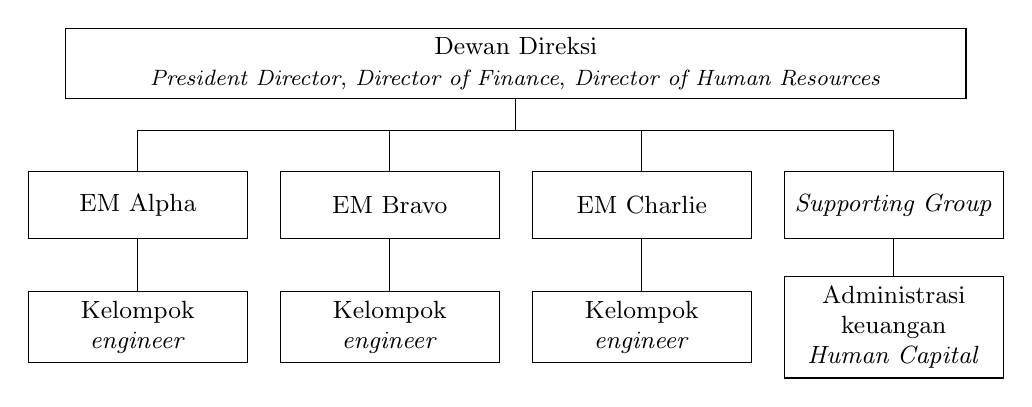
\begin{tikzpicture}[
  font=\small,
  box/.style={draw,align=center,minimum height=0.85cm,text width=2.55cm},
  line/.style={draw}]
\node[box,text width=11.2cm] (bod) at (0,0)
  {Dewan Direksi\\\footnotesize \textit{President Director}, \textit{Director of Finance}, \textit{Director of Human Resources}};
\node[box] (alpha) at (-4.8,-1.8) {EM Alpha};
\node[box] (bravo) at (-1.6,-1.8) {EM Bravo};
\node[box] (charlie) at (1.6,-1.8) {EM Charlie};
\node[box] (support) at (4.8,-1.8) {\textit{Supporting Group}};
\draw[line] (bod.south) -- (0,-0.85);
\draw[line] (-4.8,-0.85) -- (4.8,-0.85);
\foreach \name in {alpha,bravo,charlie,support}
  \draw[line] (\name.north) -- (\name.north |- 0,-0.85);
\node[box] (eng-a) at (-4.8,-3.35) {Kelompok \textit{engineer}};
\node[box] (eng-b) at (-1.6,-3.35) {Kelompok \textit{engineer}};
\node[box] (eng-c) at (1.6,-3.35) {Kelompok \textit{engineer}};
\node[box] (admin) at (4.8,-3.35) {Administrasi keuangan\\\textit{Human Capital}};
\draw[line] (alpha) -- (eng-a);
\draw[line] (bravo) -- (eng-b);
\draw[line] (charlie) -- (eng-c);
\draw[line] (support) -- (admin);
\end{tikzpicture}
